
\documentclass[12pt,a4paper]{article}

\usepackage{pdflscape}
\setlength{\textwidth}{165mm}
\setlength{\textheight}{235mm}
\setlength{\oddsidemargin}{-0mm}
\setlength{\topmargin}{-10mm}

\usepackage{mathtools}
\DeclarePairedDelimiter\abs{\lvert}{\rvert}%
\DeclarePairedDelimiter\norm{\lVert}{\rVert}%
% Swap the definition of \abs* and \norm*, so that \abs
% and \norm resizes the size of the brackets, and the
% starred version does not.
\makeatletter
\let\oldabs\abs
\def\abs{\@ifstar{\oldabs}{\oldabs*}}
%
\let\oldnorm\norm
\def\norm{\@ifstar{\oldnorm}{\oldnorm*}}
\makeatother

\newcommand*{\Value}{\frac{1}{2}x^2}%
%\usepackage{graphicx}
\usepackage{graphicx}
\usepackage{subfigure}%exclusive to subcaption
%\usepackage{subcaption, float} 
\usepackage{xcolor}
\definecolor{ggray}{RGB}{47,79,79}
\definecolor{firebrick}{RGB}{178,34,34}
\definecolor{green1}{RGB}{50,205,50}
\definecolor{umbrella}{RGB}{0,191,255}

\usepackage{pgfplots}
\usepackage{tikz}
\usetikzlibrary{patterns,arrows,shapes,positioning,shadows,trees}
\tikzstyle{every node}=[draw=black,thick,anchor=west]
\tikzstyle{selected}=[draw=red,fill=red!30]
\tikzstyle{optional}=[dashed,fill=gray!50]
\tikzstyle{neglected}=[dashed]

\usepackage{amsfonts}
\usepackage{amssymb,amsmath} %  $\displaystyle \sum$ will print a bigger one Σ , like in equations  in amsmath package

\DeclareMathOperator{\sgn}{sgn}

\usepackage{soul}

\usepackage{titlesec}
\titleformat*{\section}{\Large\sffamily}
\titleformat*{\subsection}{\large\sffamily}
\titleformat*{\subsubsection}{\itshape \sffamily}


%\renewcommand{\refname}{參考文獻}
\usepackage[nottoc]{tocbibind}
%\settocbibname{參考文獻}
\usepackage{float}
\usepackage{multirow}
\usepackage{booktabs}
%\usepackage[square]{natbib}

\title{Numerical Analysis HW10 : Spline Interpolations}
\author{Ming-Chang Chiu 100060007}
\date{\today}
\begin{document}
\maketitle
\fontsize{12}{20pt}\selectfont %本行指令第一個12是字體大小、第二個20是行距,selectfont一定要加才會發生效果。但此指令只對正文有效,註解無效

\section{Objective}
In this assignment, we are given different numbers of support points in each .dat file, with $475 \le x \le 775$. We are required to use Spline interpolation to interpolate the Y values for each $475 \le x \le 775$ and then observe the results as well as the difference between given values and interpolated values. I implemented\\ 

void splineM(int N,VEC \&X,VEC \&Y,VEC \&M)\\

double spline(double x,int N,VEC \&X,VEC \&Y,VEC \&M)\\\\
as my interpolating functions, splineM() to generate spline momentum, and spline() to calculate the interpolated value.

\section{Implementation of cubic Spline}
Cubic Spline is defined as follow:
\begin{figure}[H]
  \centering
      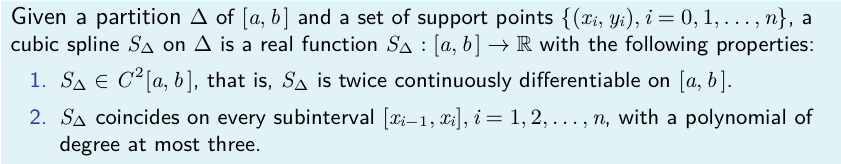
\includegraphics[width=1\textwidth]{./spline.png}
\end{figure}
and we further assume
\begin{figure}[H]
  \centering
      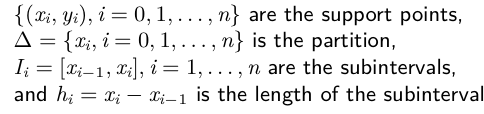
\includegraphics[width=0.4\textwidth]{./assume.png}
\end{figure}
Since $S_\Delta$ is twice continuously differentiable, we can have $$S''_{\Delta}(x) = M_{i-1}\frac{x_i - x}{h_i} + M_i \frac{x-x_i}{h_i}$$
Integrating the above equation, we have
\begin{figure}[H]
  \centering
      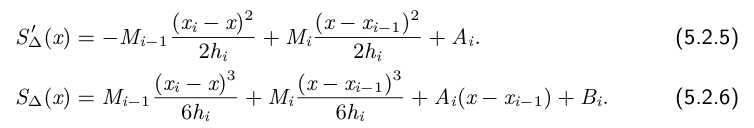
\includegraphics[width=0.7\textwidth]{./differen.png}
\end{figure}
In splineM(), I am computing the $M_i, M_{i-1}$ needed for (5.2.6) and then provide them to spline(), which exactly do what (5.2.6) is doing. 
In my code, I implement zero boundary moments as constraint in splineM(), which is $M_0 = 0$ and $M_n = 0$. Then we can get the following system of equations to solve for all moments.
\begin{figure}[H]
  \centering
      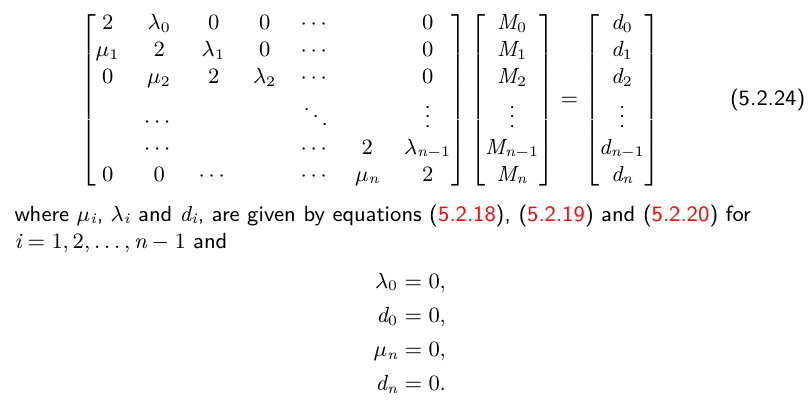
\includegraphics[width=0.7\textwidth]{./sys.png}
\end{figure}
where 
\begin{figure}[H]
  \centering
      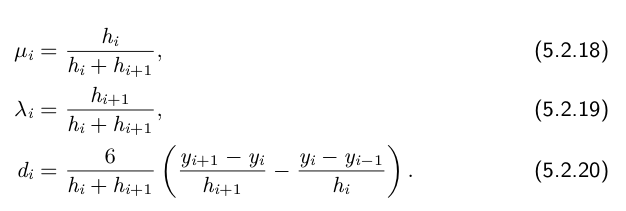
\includegraphics[width=0.7\textwidth]{./var.png}
\end{figure}
\section{Workflow}

\begin{description}  

\item [Usage:] ./hw10.out  * $<$ f*.dat, where * could be 3, 5, 7, 13, 21. For example,  ./hw10.out  3 $<$ f3.dat
\item [Solve:] Spline method is applied.
\item[Desired output:] The program will print the maximal error in [475,775] and build a file named $data.txt$, which stores value of $x_i$, interpolated value, error at $x_i$, and original value at $x_i$ in f301.dat sequentially each row. One can load the .txt file for further analysis.
\end{description}

\section{Results}
  \begin{center}
    \begin{tabular}{|c|c|c|c|}
    \hline  File & Spline's max error & Lagrange's max error&  Lagrange's max error in [500,700]\\
    \hline  f3.dat	&354.947325		&372.8669    	&372.8669	\\
    \hline  f5.dat	&190.820112		&248.3406    	&233.3644	\\
    \hline  f7.dat	&73.743612		&379.1073    	&147.5782	\\
    \hline  f13.dat	&29.044764		&1283.4489 	&39.6189	\\
    \hline  f21.dat	&19.641670		&16728.5648	& 17.804	\\\hline
 \end{tabular}

 \end{center}


\section{Plot Analysis}
The error is defined as $| Spline(x_i) - f301(x_i) |$
\begin{figure}[h!]
  \centering
      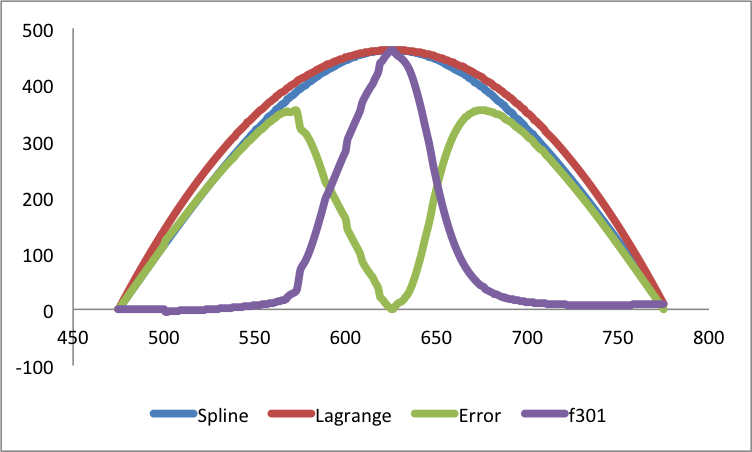
\includegraphics[width=1\textwidth]{./3.png}
  \caption{Interpolation with 3 support points}
\end{figure}
\newpage
\begin{figure}[h!]
  \centering
      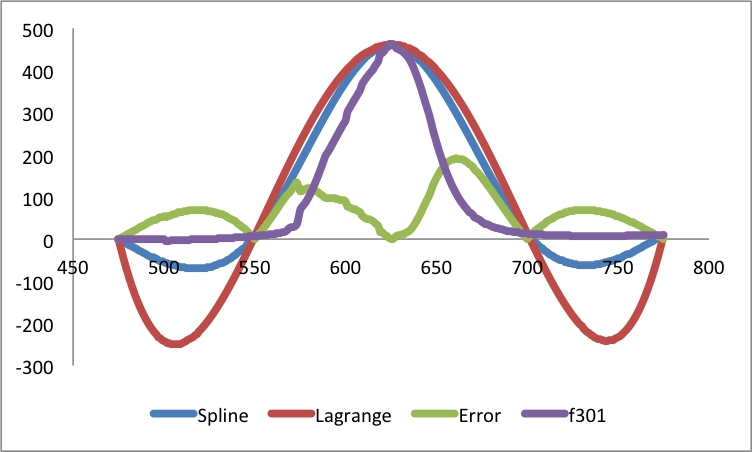
\includegraphics[width=1\textwidth]{./5.png}
  \caption{Interpolation with 5 support points}
\end{figure}
\begin{figure}[h!]
  \centering
      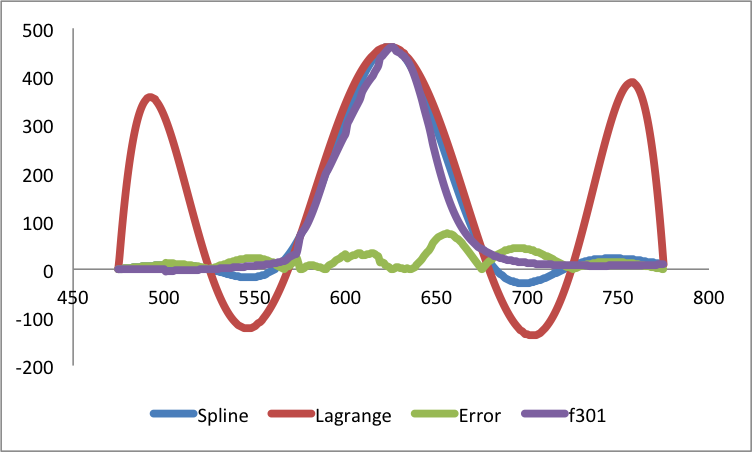
\includegraphics[width=1\textwidth]{./7.png}
  \caption{Interpolation with 7 support points}
\end{figure}
\begin{figure}[h!]
  \centering
      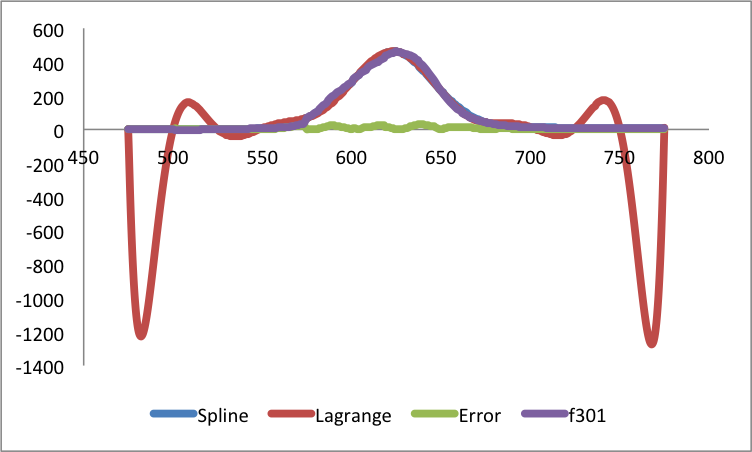
\includegraphics[width=1\textwidth]{./13.png}
  \caption{Interpolation with 13 support points}
\end{figure}
\begin{figure}[h!]
  \centering
      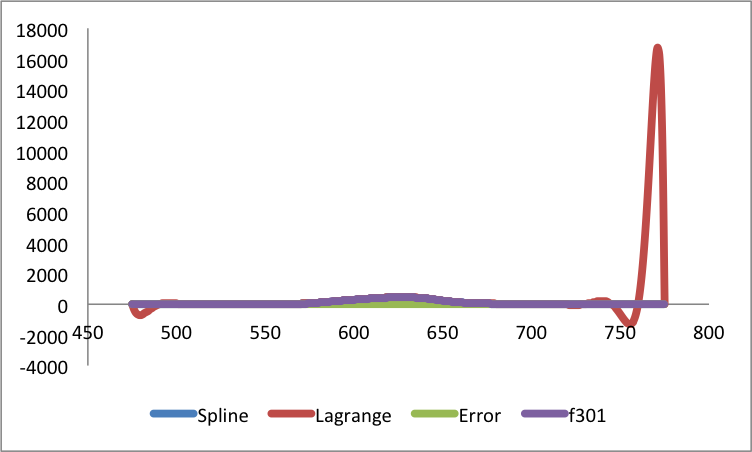
\includegraphics[width=1\textwidth]{./21.png}
  \caption{Interpolation with 21 support points}
\end{figure}
\begin{figure}[h!]
  \centering
      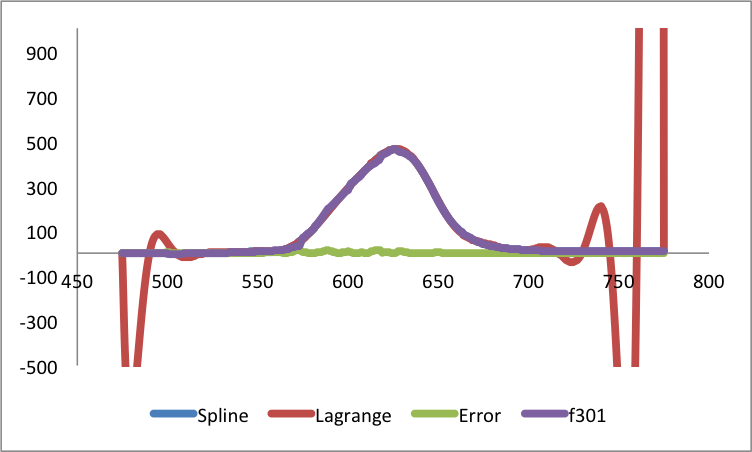
\includegraphics[width=1\textwidth]{./21_2.png}
  \caption{Interpolation with 21 support points: Magnified}
\end{figure}

\section{Observations}

In general, I would anticipate that with more support points, the more approximate the interpolated waveform will be. The result tells me my expectation is exactly true.

Compare Lagrange with Spline, we can easily observe that waveforms of Spline are a lot smoother and have massively less error at larger or small $x$. This is probably because I am using cubic spline interpolation, the order of interpolation formula is at most 3, first and second derivatives of formulae are continuous in each interval, there are much less concave and convex points in the waveforms of Spline than that of Lagrange. With smoother waveform, the error cannot be so large as Lagrange, so Spline's maximal error is then smaller.

In sum, from the table in Section 4, for all range of [475,775] the error is decreasing as more and more support points given, which means Spline will be more and more approximate to the original waveform if large amounts of support points are provided. The reason may reside in that since 1st and 2nd derivatives of cubic Spline functions are continuous, the interpolated waveform will be smooth, with more equal spaced subintervals(i.e. more support points) the interpolated values will be more approximate to f301.

\end{document} 
